\chapter{Methodology}
\label{ch:methodology}

\section{Introduction}
\label{sec:3.1}

This chapter sets out how the CFL-EDLSTM framework introduced in Chapter~1 and motivated by the gaps identified in Chapter~2 was actually built. It starts with the overall research design and a high-level picture of the proposed framework, then narrows into the concrete details: the study area, the 26 monitoring stations, where the data came from, what the five variables actually look like, how the raw records were cleaned and aligned, how the stations were grouped into clusters, and how the time-series inputs and forecasting horizons were set up. The architecture itself, the baseline models, the evaluation design, the SHAP procedure, and the visualization platform are covered in the sections that follow this one.

% ------------------------------------------------------------
\section{Research Design}
\label{sec:3.2}

This is a quantitative, experimental study built around a comparative design: one proposed framework (CFL-EDLSTM) evaluated against four baseline architectures, across four station clusters and seven forecasting horizons, using historical observational data rather than data generated for the purpose of the study. The work is applied rather than purely theoretical --- the goal is a forecasting system that could plausibly be used, not just a proof of concept --- which is also why a web-based visualization platform and an external comparison against FFWC are part of the design rather than an afterthought.

% ------------------------------------------------------------
\section{Overall Proposed Framework}
\label{sec:3.3}

At its core, the framework combines two ideas that Chapter~2 examined separately: a sequence-to-sequence Encoder--Decoder LSTM for multi-step forecasting \cite{Kao2020,Cui2022}, and a clustered federated training procedure in which stations are grouped by hydrological similarity and each group trains its own model via Federated Averaging \cite{McMahan2017,Ghosh2021,Harshvardhan2022}. Rather than pooling every station's data into one central model, each of the 26 stations trains locally within its assigned cluster, and only model parameters --- never raw station data --- are shared and aggregated.

\vspace{0.3cm}
\begin{figure}[htbp]
    \centering
    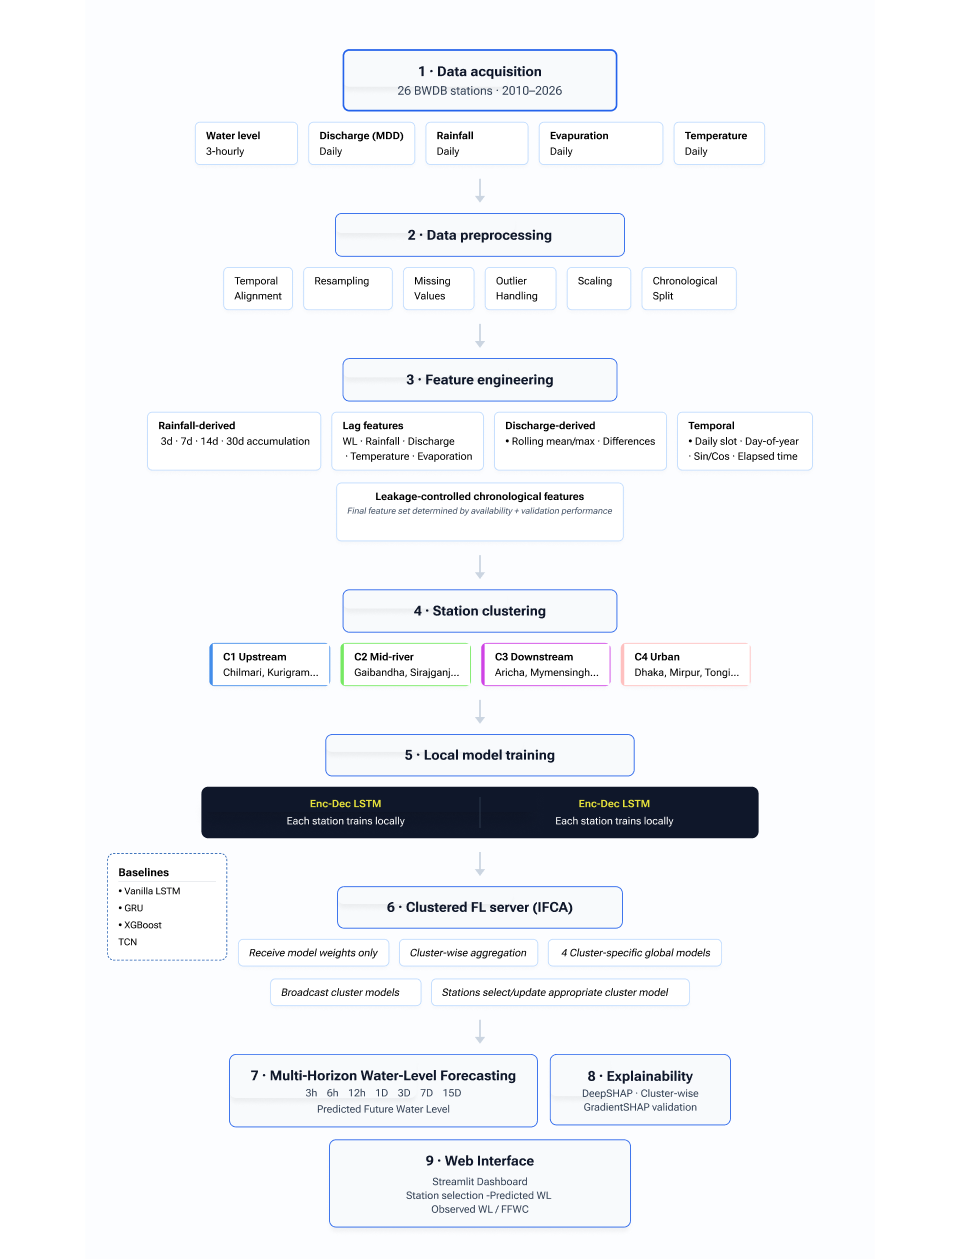
\includegraphics[
        width=0.92\textwidth
    ]{figures2/fig3-1-framework.png}

    \caption{Overall CFL-EDLSTM framework diagram.}
    \label{fig:3.1}
\end{figure}

% ------------------------------------------------------------
\section{Study Area}
\label{sec:3.4}

The study covers 25 water-level monitoring stations distributed across northern, central, western, and Dhaka-metropolitan parts of Bangladesh, spanning a network of 13 named river systems: the Teesta and Dharla in the north; the Deonai-Charalkata-Jamuneswari-Karatoa system; the Brahmaputra-Jamuna mainstem, which contains the largest number of monitoring stations in the study; the Ghagot; the Old Brahmaputra; the interconnected Karatoa-Atrai-Gur-Gumani-Hurasagar system; the Dhaleswari and Kaliganga-Bethua further downstream; and, around the greater Dhaka area, the Buriganga, Turag, Lakhya, and Balu.
BWDB classifies each station as tidal or non-tidal: 5 of the 25 stations, all of them in the Urban cluster and located on the Buriganga, Turag, Lakhya, and Balu channels around Dhaka, are tidal; the remaining 20 are non-tidal. This distinction is reported here as descriptive context about the study area rather than as a formal input to the clustering procedure itself, which is defined separately in \S\ref{sec:3.10.1}.

\setcounter{table}{-1}
\begin{table}[htbp]
  \centering
  \caption{River System Distribution}
  \label{tab:3.0}
  \small
  \begin{tabular}{@{}L{5.0cm} C{1.7cm} L{3.8cm} L{2.2cm}@{}}
    \toprule
    \textbf{River System} & \textbf{No. of Stations} & \textbf{General Location} & \textbf{Tidal Status} \\
    \midrule
    Teesta & 2 & Northern Bangladesh & Non-tidal \\
    Dharla & 1 & Northern Bangladesh & Non-tidal \\
    Deonai--Charalkata--Jamuneswari--Karatoa & 3 & Northern Bangladesh & Non-tidal \\
    Brahmaputra--Jamuna & 6 & Northern and central Bangladesh & Non-tidal \\
    Ghagot & 1 & Northern Bangladesh & Non-tidal \\
    Old Brahmaputra & 2 & Central Bangladesh & Non-tidal \\
    Karatoa--Atrai--Gur--Gumani--Hurasagar & 2 & Central and downstream Bangladesh & Non-tidal \\
    Dhaleswari & 2 & Central and downstream Bangladesh & Non-tidal \\
    Kaliganga--Bethua & 1 & Central and downstream Bangladesh & Non-tidal \\
    Buriganga & 1 & Greater Dhaka & Tidal \\
    Turag & 1 & Greater Dhaka & Tidal \\
    Lakhya & 2 & Greater Dhaka & Tidal \\
    Balu & 1 & Greater Dhaka & Tidal \\
    \midrule
    \textbf{Total} & \textbf{25} & \textbf{Bangladesh} & \textbf{20 Non-tidal / 5 Tidal} \\
    \bottomrule
  \end{tabular}
\end{table}


\begin{figure}[htbp]
    \centering
    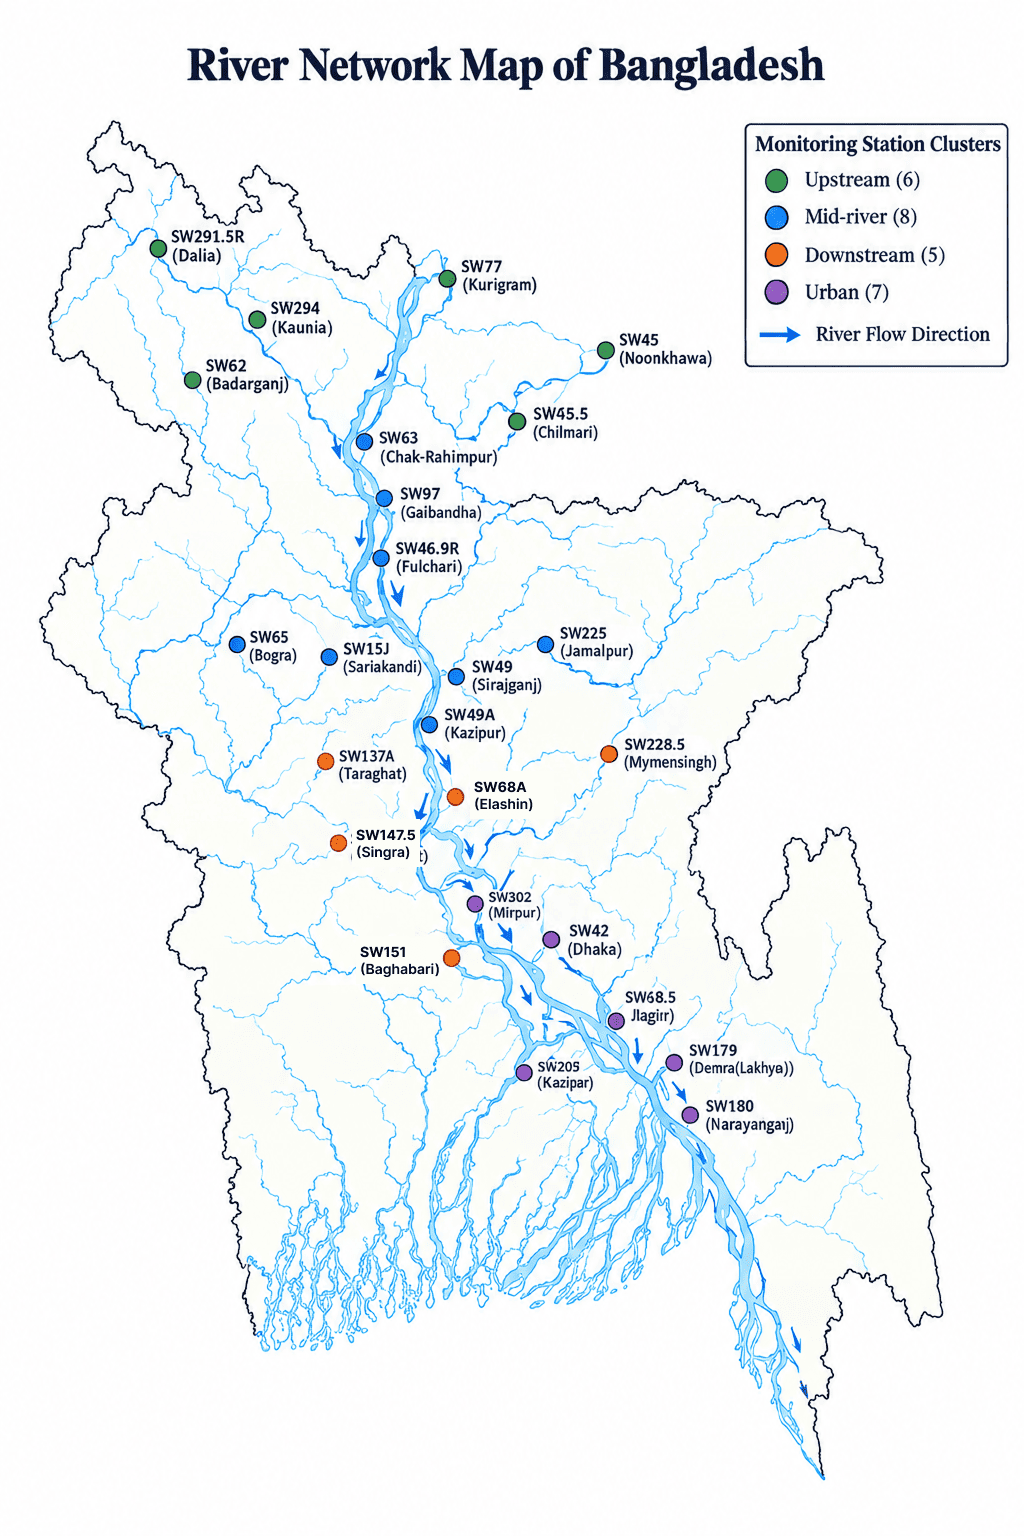
\includegraphics[
        width=0.85\textwidth
    ]{figures2/fig3-2a-river-connectivity.png}

    \caption{River system connectivity within the study area.}
    \label{fig:3.2a}
\end{figure}

\begin{figure}[htbp]
    \centering
    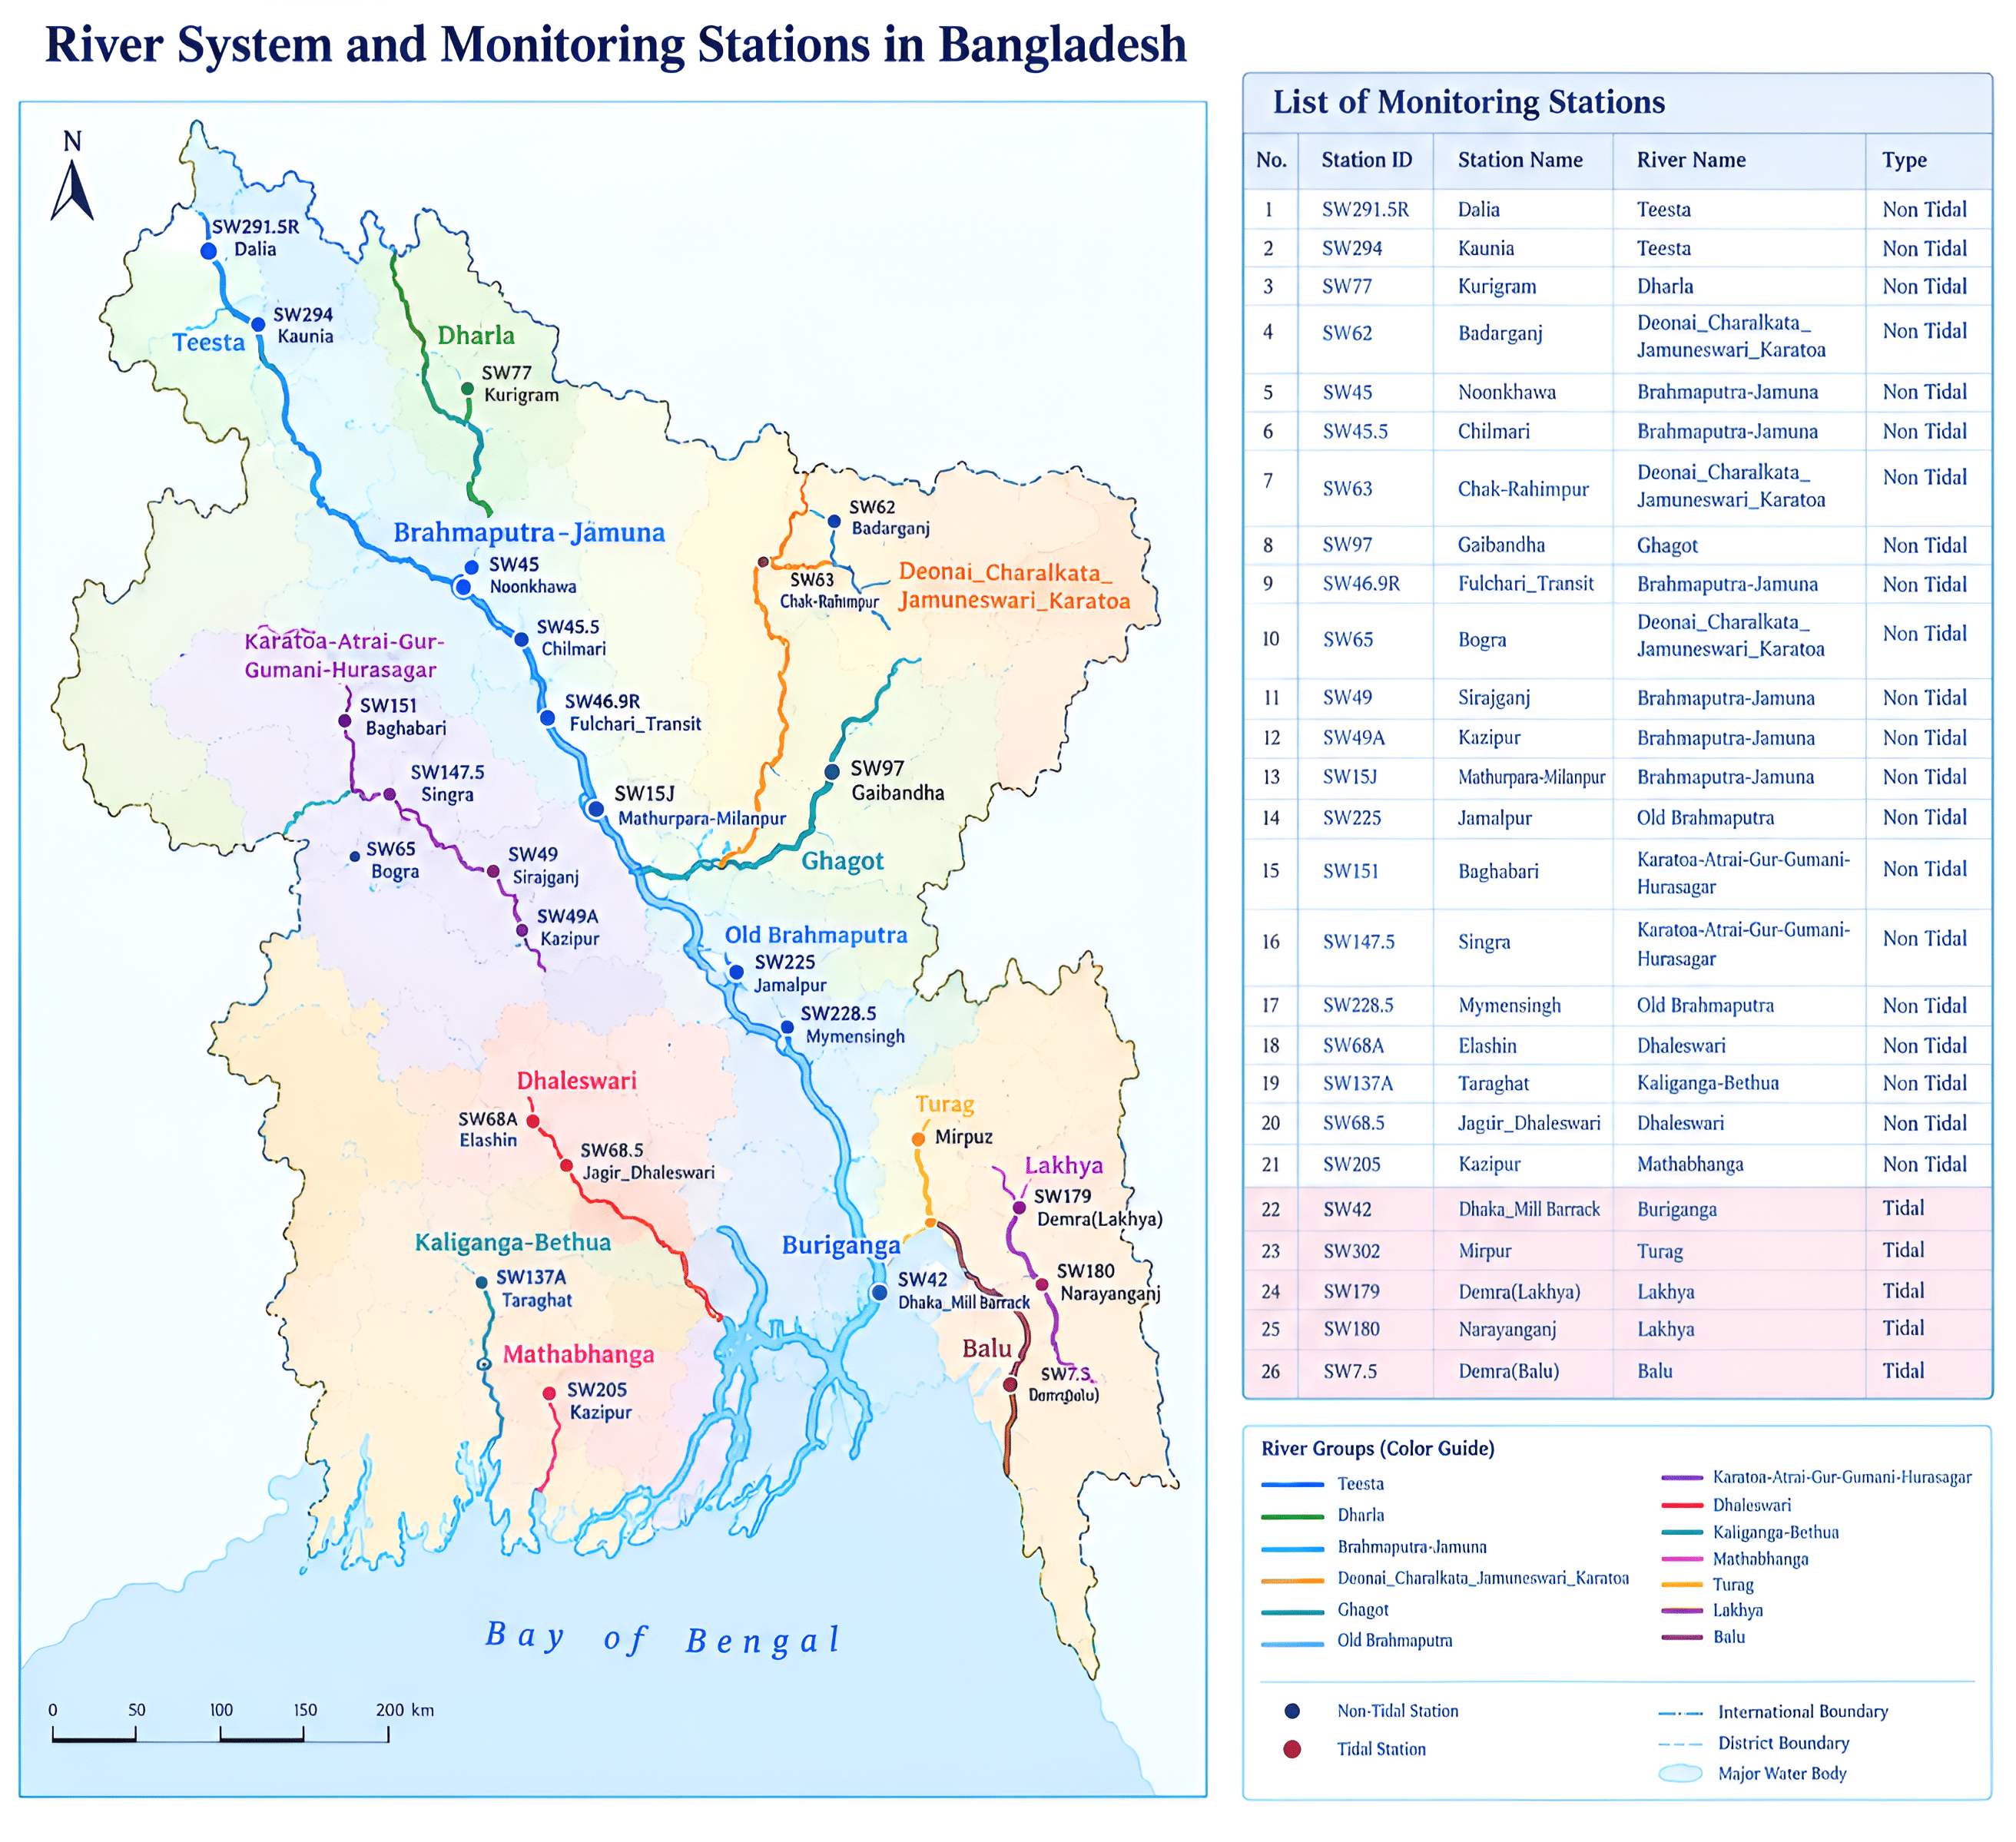
\includegraphics[
        width=0.75\textwidth
    ]{figures2/fig3-2b-station-distribution.png}

    \caption{Geographical distribution of the 25 monitoring stations.}
    \label{fig:3.2b}
\end{figure}

% ------------------------------------------------------------
\section{Monitoring Stations}
\label{sec:3.5}

Water level is the variable with the widest coverage in this study and effectively defines the station network: 25 stations report water level, and every other variable is a subset of that same 25. Table~\ref{tab:3.1} lists them.

\begin{landscape}
\begin{table}[htbp]
  \centering
  \caption{Station Inventory}
  \label{tab:3.1}
  \scriptsize
  \setlength{\tabcolsep}{3pt}
  \begin{tabularx}{\linewidth}{@{}c l X X l X X r r l@{}}
    \toprule
    \textbf{\#} & \textbf{Station ID} & \textbf{Station Name} & \textbf{River} & \textbf{Type} &
    \textbf{District} & \textbf{Upazila} & \textbf{Lat} & \textbf{Long} & \textbf{Cluster} \\
    \midrule
    1 & SW291.5R & Dalia & Teesta & Non-Tidal & Nilphamari & Dimla & 26.176 & 89.051 & Upstream \\
    2 & SW294 & Kaunia & Teesta & Non-Tidal & Rangpur & Kaunia & 25.789 & 89.439 & Upstream \\
    3 & SW77 & Kurigram & Dharla & Non-Tidal & Kurigram & Kurigram Sadar & 25.823 & 89.665 & Upstream \\
    4 & SW62 & Badarganj & Deonai-Charalkata-Jamuneswari-Karatoa & Non-Tidal & Rangpur & Badarganj & 25.682 & 89.076 & Upstream \\
    5 & SW45 & Noonkhawa & Brahmaputra-Jamuna & Non-Tidal & Kurigram & Kurigram Sadar & 25.920 & 89.770 & Upstream \\
    6 & SW45.5 & Chilmari & Brahmaputra-Jamuna & Non-Tidal & Kurigram & Chilmari & 25.568 & 89.679 & Upstream \\
    7 & SW63 & Chak-Rahimpur & Deonai-Charalkata-Jamuneswari-Karatoa & Non-Tidal & Gaibandha & Gobindaganj & 25.147 & 89.360 & Middle \\
    8 & SW97 & Gaibandha & Ghagot & Non-Tidal & Gaibandha & Gaibandha Sadar & 25.339 & 89.551 & Middle \\
    9 & SW46.9R & Fulchari (Transit) & Brahmaputra-Jamuna & Non-Tidal & Gaibandha & Fulchhari & 25.187 & 89.599 & Middle \\
    10 & SW65 & Bogra & Deonai-Charalkata-Jamuneswari-Karatoa & Non-Tidal & Bogura & Bogura Sadar & 24.846 & 89.379 & Middle \\
    11 & SW49 & Sirajganj & Brahmaputra-Jamuna & Non-Tidal & Sirajganj & Sirajganj Sadar & 24.468 & 89.720 & Middle \\
    12 & SW49A & Kazipur & Brahmaputra-Jamuna & Non-Tidal & Sirajganj & Kazipur & 24.670 & 89.649 & Middle \\
    13 & SW15J & Mathurpara-Milanpur & Brahmaputra-Jamuna & Non-Tidal & Bogura & Shariakandi & 24.837 & 89.587 & Middle \\
    14 & SW225 & Jamalpur & Old Brahmaputra & Non-Tidal & Jamalpur & Jamalpur Sadar & 24.922 & 89.968 & Middle \\
    15 & SW151 & Baghabari & Karatoa-Atrai-Gur-Gumani-Hurasagar & Non-Tidal & Sirajganj & Shahjadpur & 24.131 & 89.581 & Downstream \\
    16 & SW147.5 & Singra & Karatoa-Atrai-Gur-Gumani-Hurasagar & Non-Tidal & Natore & Singra & 24.498 & 89.139 & Downstream \\
    17 & SW228.5 & Mymensingh & Old Brahmaputra & Non-Tidal & Mymensingh & Mymensingh Sadar & 24.737 & 90.430 & Downstream \\
    18 & SW68A & Elashin & Dhaleswari & Non-Tidal & Tangail & Delduar & 24.119 & 89.888 & Downstream \\
    19 & SW137A & Taraghat & Kaliganga-Bethua & Non-Tidal & Manikganj & Ghior & 23.858 & 89.956 & Downstream \\
    20 & SW68.5 & Jagir (Dhaleswari) & Dhaleswari & Non-Tidal & Manikganj & Manikganj Sadar & 23.879 & 90.025 & Urban \\
    21 & SW42 & Dhaka (Mill Barrack) & Buriganga & Tidal & Dhaka & Dhaka Sadar (Kotwali) & 23.697 & 90.420 & Urban \\
    22 & SW302 & Mirpur & Turag & Tidal & Dhaka & Mirpur & 23.785 & 90.336 & Urban \\
    23 & SW179 & Demra (Lakhya) & Lakhya & Tidal & Dhaka & Demra & 23.728 & 90.506 & Urban \\
    24 & SW180 & Narayanganj & Lakhya & Tidal & Narayanganj & Narayanganj Sadar & 23.630 & 90.515 & Urban \\
    25 & SW7.5 & Demra (Balu) & Balu & Tidal & Dhaka & Demra & 23.733 & 90.496 & Urban \\
    \bottomrule
  \end{tabularx}
\end{table}
\end{landscape}




% \begin{figure}[htbp]
%     \centering

%     \includegraphics[
%         width=0.85\textwidth
%     ]{figures/fig3-3-cluster-map.png}

%     \caption{25-station, four-cluster spatial map of Bangladesh.}
%     \label{fig:3.3}
% \end{figure}

% ------------------------------------------------------------
\section{Data Sources}
\label{sec:3.6}

\begin{landscape}
\begin{table}[htbp]
  \centering
  \caption{Data Sources by Variable}
  \label{tab:3.2}
  \footnotesize
  \setlength{\tabcolsep}{4pt}
  \renewcommand{\arraystretch}{1.25}
  \begin{tabularx}{\linewidth}{@{}L{2.0cm} L{1.3cm} L{1.9cm} X L{2.2cm} L{1.3cm}@{}}
    \toprule
    \textbf{Variable} & \textbf{Source} & \textbf{Station Coverage} &
    \textbf{How Used} & \textbf{Collection Period} & \textbf{Unit} \\
    \midrule
    Water Level & BWDB gauge stations & 25 stations &
    Retained at native 5-obs/day resolution as the study's master timeline (\S\ref{sec:3.9.3}) &
    1 Jan 2010 -- 31 Mar 2026 & WL (mMSL) \\

    Discharge & BWDB & 15 stations &
    Used directly + trend features; mapped across the 5 WL slots per date &
    1 Jan 2010 -- 31 Dec 2024 & MDD (m\textsuperscript{3}/s) \\

    Rainfall & BWDB / BMD & 13 stations &
    Used directly + cumulative windows; mapped across the 5 WL slots per date &
    1 Jan 2010 -- $\sim$30 Apr 2026 & mm \\

    Temperature & Mendeley dataset + NASA POWER & 11 districts (district-level) &
    Gaps filled via interpolation, mapped to stations by district, then mapped across the 5 WL slots &
    2012 -- 2024 & \textdegree C \\

    Evaporation & BWDB & 7 stations (station-level) &
    Linearly interpolated to fill gaps; mapped across the 5 WL slots per date &
    1 Jan 2010 -- 28 Feb 2026 & mm/day \\
    \bottomrule
  \end{tabularx}
\end{table}
\end{landscape}

Not every station carries every variable. Water level has by far the widest footprint, at 25 stations; evaporation is the narrowest, at 7. Temperature is district-level rather than station-level, so it has to be mapped onto individual stations by district rather than read directly from a gauge --- this is discussed further in \S\ref{sec:3.9.1} and \S\ref{sec:3.9.3}.

% ------------------------------------------------------------
\section{Dataset Description}
\label{sec:3.7}

Across the five variables, the dataset totals 1,092,687 raw observations before any cleaning or alignment: 762,813 for water level, 46,812 for discharge, 71,110 for rainfall, 40,761 for evaporation, and 171,191 for temperature. Water level's much larger share reflects both its wider station coverage and its finer native resolution (5 observations/day, against daily for discharge, rainfall, temperature, and evaporation).

Coverage across variables is genuinely uneven rather than a uniform grid. Of the 13 districts represented anywhere in the dataset, only four --- Bogura, Dhaka, Rangpur, and Sirajganj --- have all five variables present. Most districts have three or four, and one (Narayanganj) have only water level and one other variable. This unevenness is exactly why station clustering (\S\ref{sec:3.10}) and careful preprocessing (\S\ref{sec:3.9}) matter as much as they do here --- a model can't assume every station looks like every other station going in.

% ------------------------------------------------------------
\section{Input and Target Variables}
\label{sec:3.8}

Five variables make up the modeling input, one of which --- water level --- is also the forecasting target. Combining them this way directly answers the single-variable limitation flagged repeatedly in Chapter~2 \cite{Islam2026b,Ruma2023,Rakin2023,HemelSakib2024}, none of which brought discharge, water level, rainfall, temperature, and evaporation together in one framework.

\begin{table}[htbp]
  \centering
  \caption{Input and Target Variables}
  \label{tab:3.3}
  \small
  \renewcommand{\arraystretch}{1.2}
  \setlength{\tabcolsep}{5pt}
  \begin{tabular}{@{}L{2.1cm} L{2.2cm} L{4.0cm} L{2.7cm} L{1.7cm}@{}}
    \toprule
    \textbf{Variable} & \textbf{Type} & \textbf{Original Resolution} & \textbf{Role} & \textbf{Unit} \\
    \midrule
    Water Level & Hydrological & 3-hourly, 5 obs/day (06:00--18:00) & Target (and input, via lag) & mMSL \\
    Discharge & Hydrological & Daily (mean) & Input & m\textsuperscript{3}/s (MDD) \\
    Rainfall & Meteorological & Daily & Input & mm \\
    Temperature & Meteorological & Daily (district-level) & Input & \textdegree C \\
    Evaporation & Meteorological & Daily (with gaps) & Input & mm/day \\
    \bottomrule
  \end{tabular}
\end{table}

\subsection{Water Level}
\label{sec:3.8.1}

Water level is the target variable throughout this thesis. It is recorded at 25 BWDB gauge stations five times a day --- 06:00, 09:00, 12:00, 15:00, and 18:00, three hours apart during the day with a twelve-hour gap overnight --- the finest native resolution of any variable in the dataset, and it is retained at that native resolution as the study's master modelling timeline (\S\ref{sec:3.9.3}), rather than being collapsed down to a single daily value. Measured in metres above mean sea level (mMSL), it is the quantity every forecast horizon in this thesis ultimately predicts, following the same target-variable choice made by \cite{Ruma2023} and, for a smaller station set, \cite{Islam2026b}.

\subsection{Discharge}
\label{sec:3.8.2}

Discharge (mean daily discharge, MDD) is recorded at 15 of the 25 stations, in cubic metres per second, and used both directly and through derived trend features. Discharge is the input variable \cite{Islam2026a} relied on exclusively for their Old Brahmaputra forecasting work --- and one of the two limitations they themselves flagged was the exclusion of exactly the kind of meteorological variables (rainfall, temperature) this thesis adds alongside it.

\subsection{Rainfall}
\label{sec:3.8.3}

Rainfall is recorded daily at 13 stations, in millimetres, and used both directly and as cumulative windows to capture delayed catchment response. This mirrors the lag-based and cumulative-rainfall treatment used by \cite{Islam2026b} and the areal-rainfall approach of \cite{Cui2022}, both of which found rainfall to carry real, if secondary, predictive weight relative to antecedent discharge or water level.

\subsection{Temperature}
\label{sec:3.8.4}

Temperature is the one variable in this dataset that is not station-specific: it comes from a combination of a Mendeley dataset and NASA POWER reanalysis data, at daily resolution, covering 11 districts, with gaps filled via interpolation and values mapped onto stations by district. Because temperature is district-level rather than station-level, it still carries less direct/observational weight than the station-specific variables, and any gap-filling interpolation should be treated with the same caution as elsewhere in the dataset --- worth being explicit about in any later discussion of SHAP-based feature importance (\S3.16 / Chapter~4), since a variable mapped from district to station shouldn't be interpreted quite the same way as one measured directly at the station.

\subsection{Evaporation}
\label{sec:3.8.5}

Evaporation is recorded daily at 7 stations --- the narrowest coverage of any variable --- and, like temperature, is linearly interpolated to daily values where gaps exist. Its inclusion follows the precedent of \cite{Cui2022}, who found that adding evaporation alongside rainfall improved multi-step forecasting accuracy in their Encoder--Decoder framework, even though its coverage in that study was similarly narrower than the other inputs.

% ------------------------------------------------------------
\section{Data Preprocessing}
\label{sec:3.9}

\begin{figure}[htbp]
    \centering

    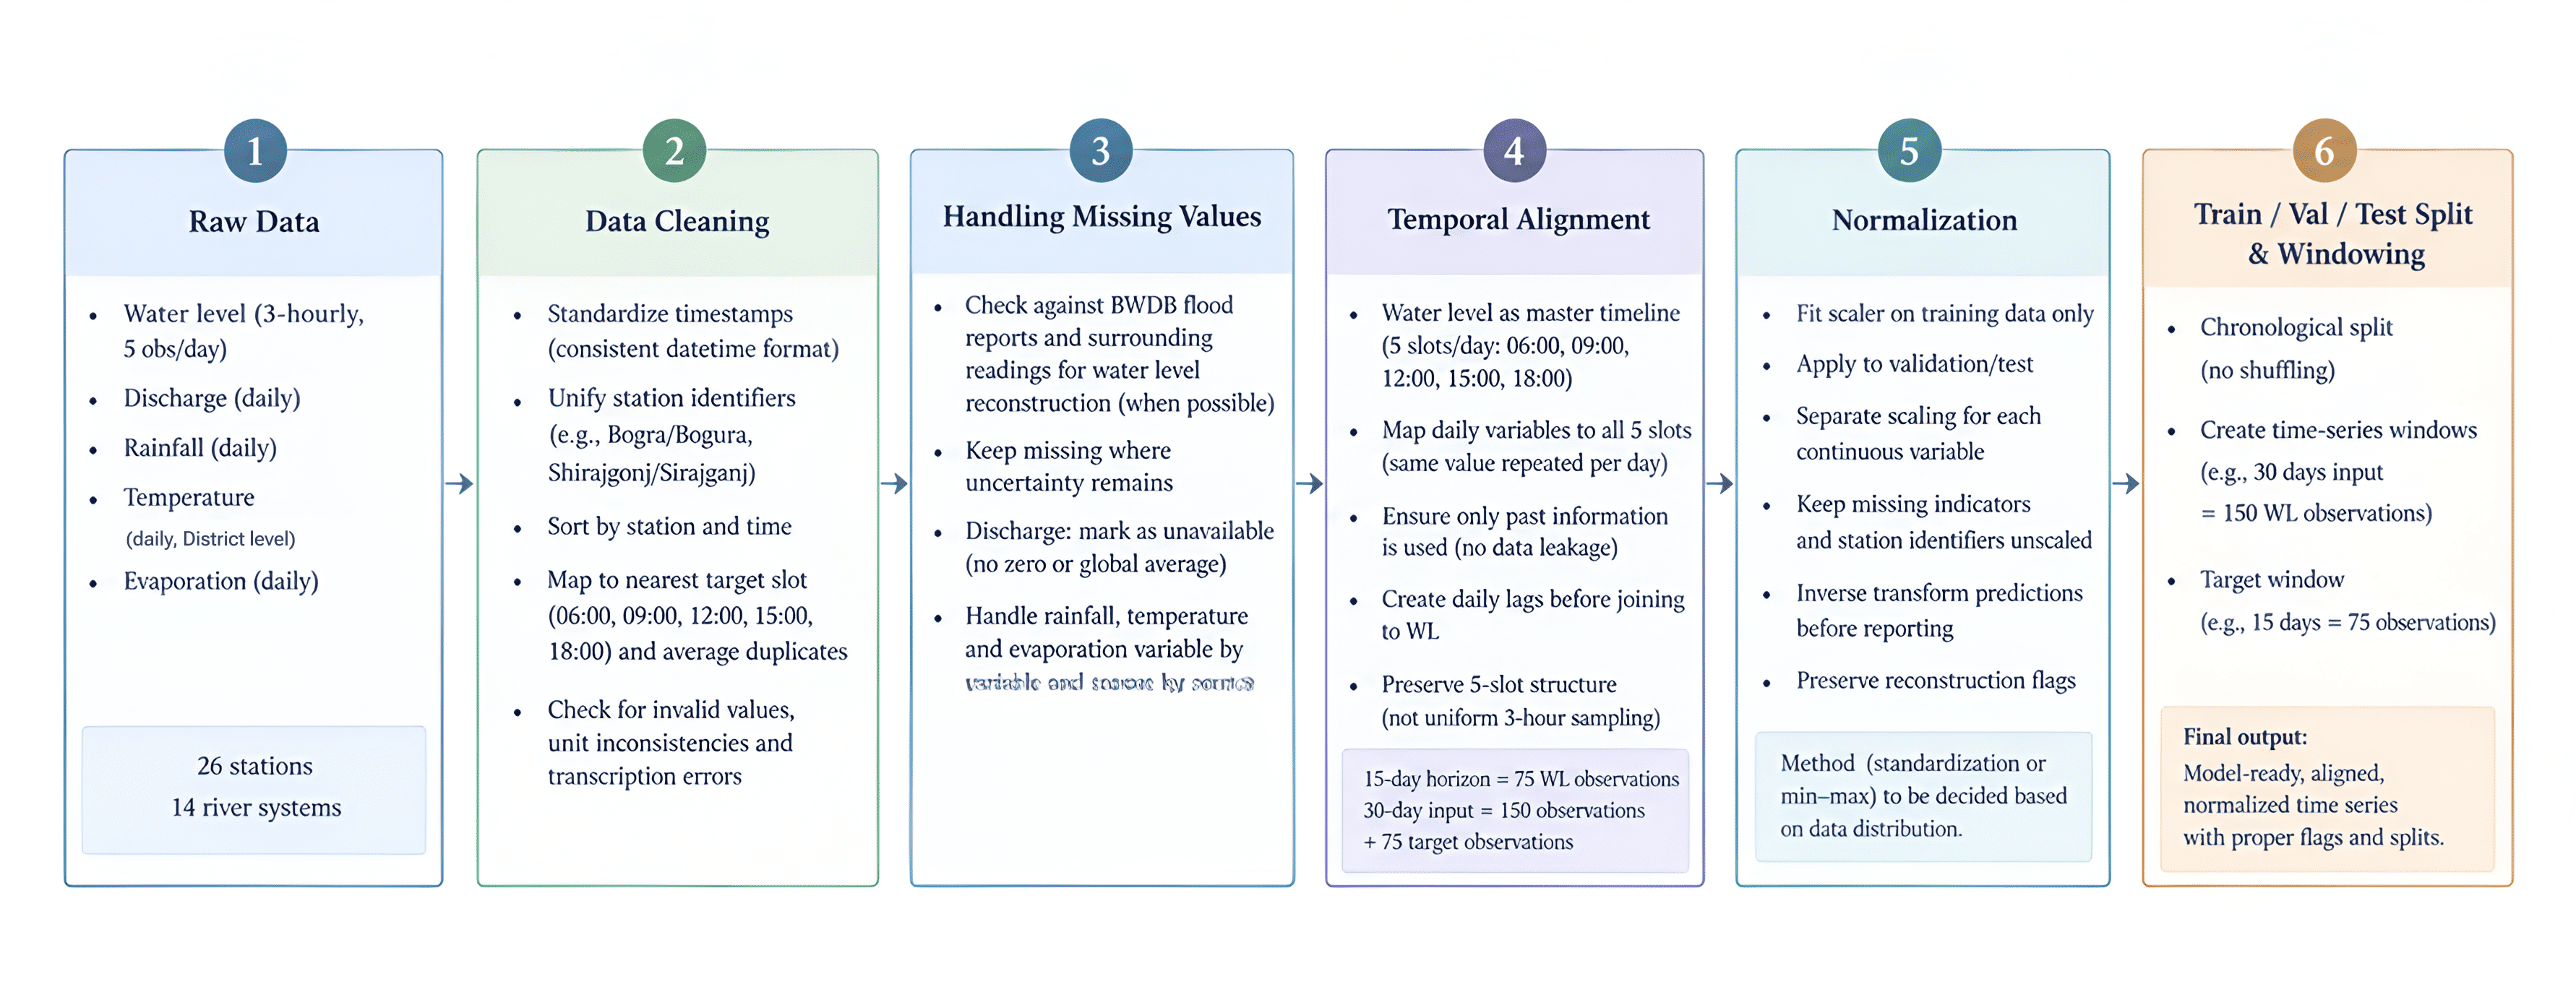
\includegraphics[
        width=0.9\textwidth
    ]{figures2/fig3-4-preprocessing-pipeline.png}

    \caption{Data preprocessing pipeline flowchart.}
    \label{fig:3.4}
\end{figure}

\subsection{Data Cleaning}
\label{sec:3.9.1}

Before anything else, timestamps across all five sources are parsed into one consistent datetime format, station identifiers are standardized against the naming inconsistencies already flagged in \S\ref{sec:3.5} (Bogra/Bogura, Shirajgonj/Sirajganj, and similar), and every record is sorted by station and time. Water-level readings are mapped to the nearest of the five target slots --- 06:00, 09:00, 12:00, 15:00, or 18:00 --- by closest value alone, with no separate tolerance threshold applied. Where more than one reading lands in the same station-slot, they're combined by taking the mean. Duplicate records, impossible numeric values, inconsistent units, and likely transcription errors are all checked for --- but extreme water-level values are inspected rather than dropped automatically, since an extreme reading during this kind of study is just as likely to be a real flood as it is to be an error.

Before any of the four supporting variables get merged in, the station metadata itself is checked. Rainfall, temperature, and evaporation are assigned to the 25 water-level stations primarily by district match --- whatever district a station is recorded under is used to find the corresponding rainfall/temperature/evaporation source for that same district --- and where no matching source exists in that station's own district, the nearest available station geographically is used instead. Discharge (MDD) is mapped directly to its corresponding water-level station wherever a measurement exists. Which source gauge fed which station is kept on record throughout, rather than discarded once the merge is done.

\subsection{Handling Missing Values}
\label{sec:3.9.2}

Missing water-level readings aren't treated as random noise. A large share of them are almost certainly tied to flooding itself, since gauges can fail or go unread precisely when water levels spike --- which means the gaps that matter most are exactly the ones a careless imputation method would handle worst. Where a gap coincides with a known event, it's checked against BWDB flood reports and the surrounding water-level trajectory at that station, and only reconstructed where both the report and the neighboring readings genuinely support a specific value --- with reconstructed points flagged separately from directly observed ones from that point on. Where the evidence isn't strong enough to reconstruct with any confidence, the gap stays marked as missing rather than being papered over.

Discharge is handled more conservatively, since it maps directly to specific stations and simply isn't available at all of them. A missing MDD value is recorded as unavailable, never as zero, and is never filled in from a global average or borrowed from another station. Gaps in rainfall, temperature, and evaporation are handled on the same principle --- assessed variable by variable and source by source.

One station needs an explicit note rather than silent handling: the Narayanganj Sadar rainfall record contains only 61 entries, against roughly 5,900 for every other rainfall station. It is retained in the dataset --- removing it now would require re-touching totals and figures already finalized elsewhere in this thesis, and no alternative or supplementary source is currently available for it --- but its extremely limited coverage means it should be treated with caution in any rainfall-dependent feature or result specific to that station, and this limitation is stated explicitly here rather than left for a reader to discover on their own.

\subsection{Temporal Alignment}
\label{sec:3.9.3}

Water level defines the modelling timeline here, at its native five-observations-a-day schedule (06:00, 09:00, 12:00, 15:00, 18:00), rather than being collapsed down to a single daily value. The four supporting variables --- rainfall, temperature, evaporation, and discharge --- are all daily, so each one is mapped to its corresponding station and matched by date across all five of that date's water-level slots; a given day's rainfall total, for instance, appears identically in all five rows for that date. That repetition is there to align the feature matrix, not to imply five independent rainfall measurements were actually taken.

The definition and reporting window of each daily variable are checked before use. A daily total that includes measurements occurring after a WL prediction time must not be treated as already known at that time. Inputs must reflect only information available at the forecast origin. Where suitable, daily lags are generated by shifting the original daily series by calendar days before joining it to WL, rather than shifting rows in the expanded five-observation dataset.

Daytime observations are approximately three hours apart, but the interval from 18:00 to the following 06:00 is twelve hours. The series is therefore not uniformly sampled every three hours. Preprocessing preserves the five-slot daily structure or represents elapsed time explicitly where supported by the model. A 15-day horizon corresponds to 75 WL observations; for example, a 30-day input window contains 150 WL observations followed by a 75-observation target.


\begin{figure}[htbp]
    \centering

    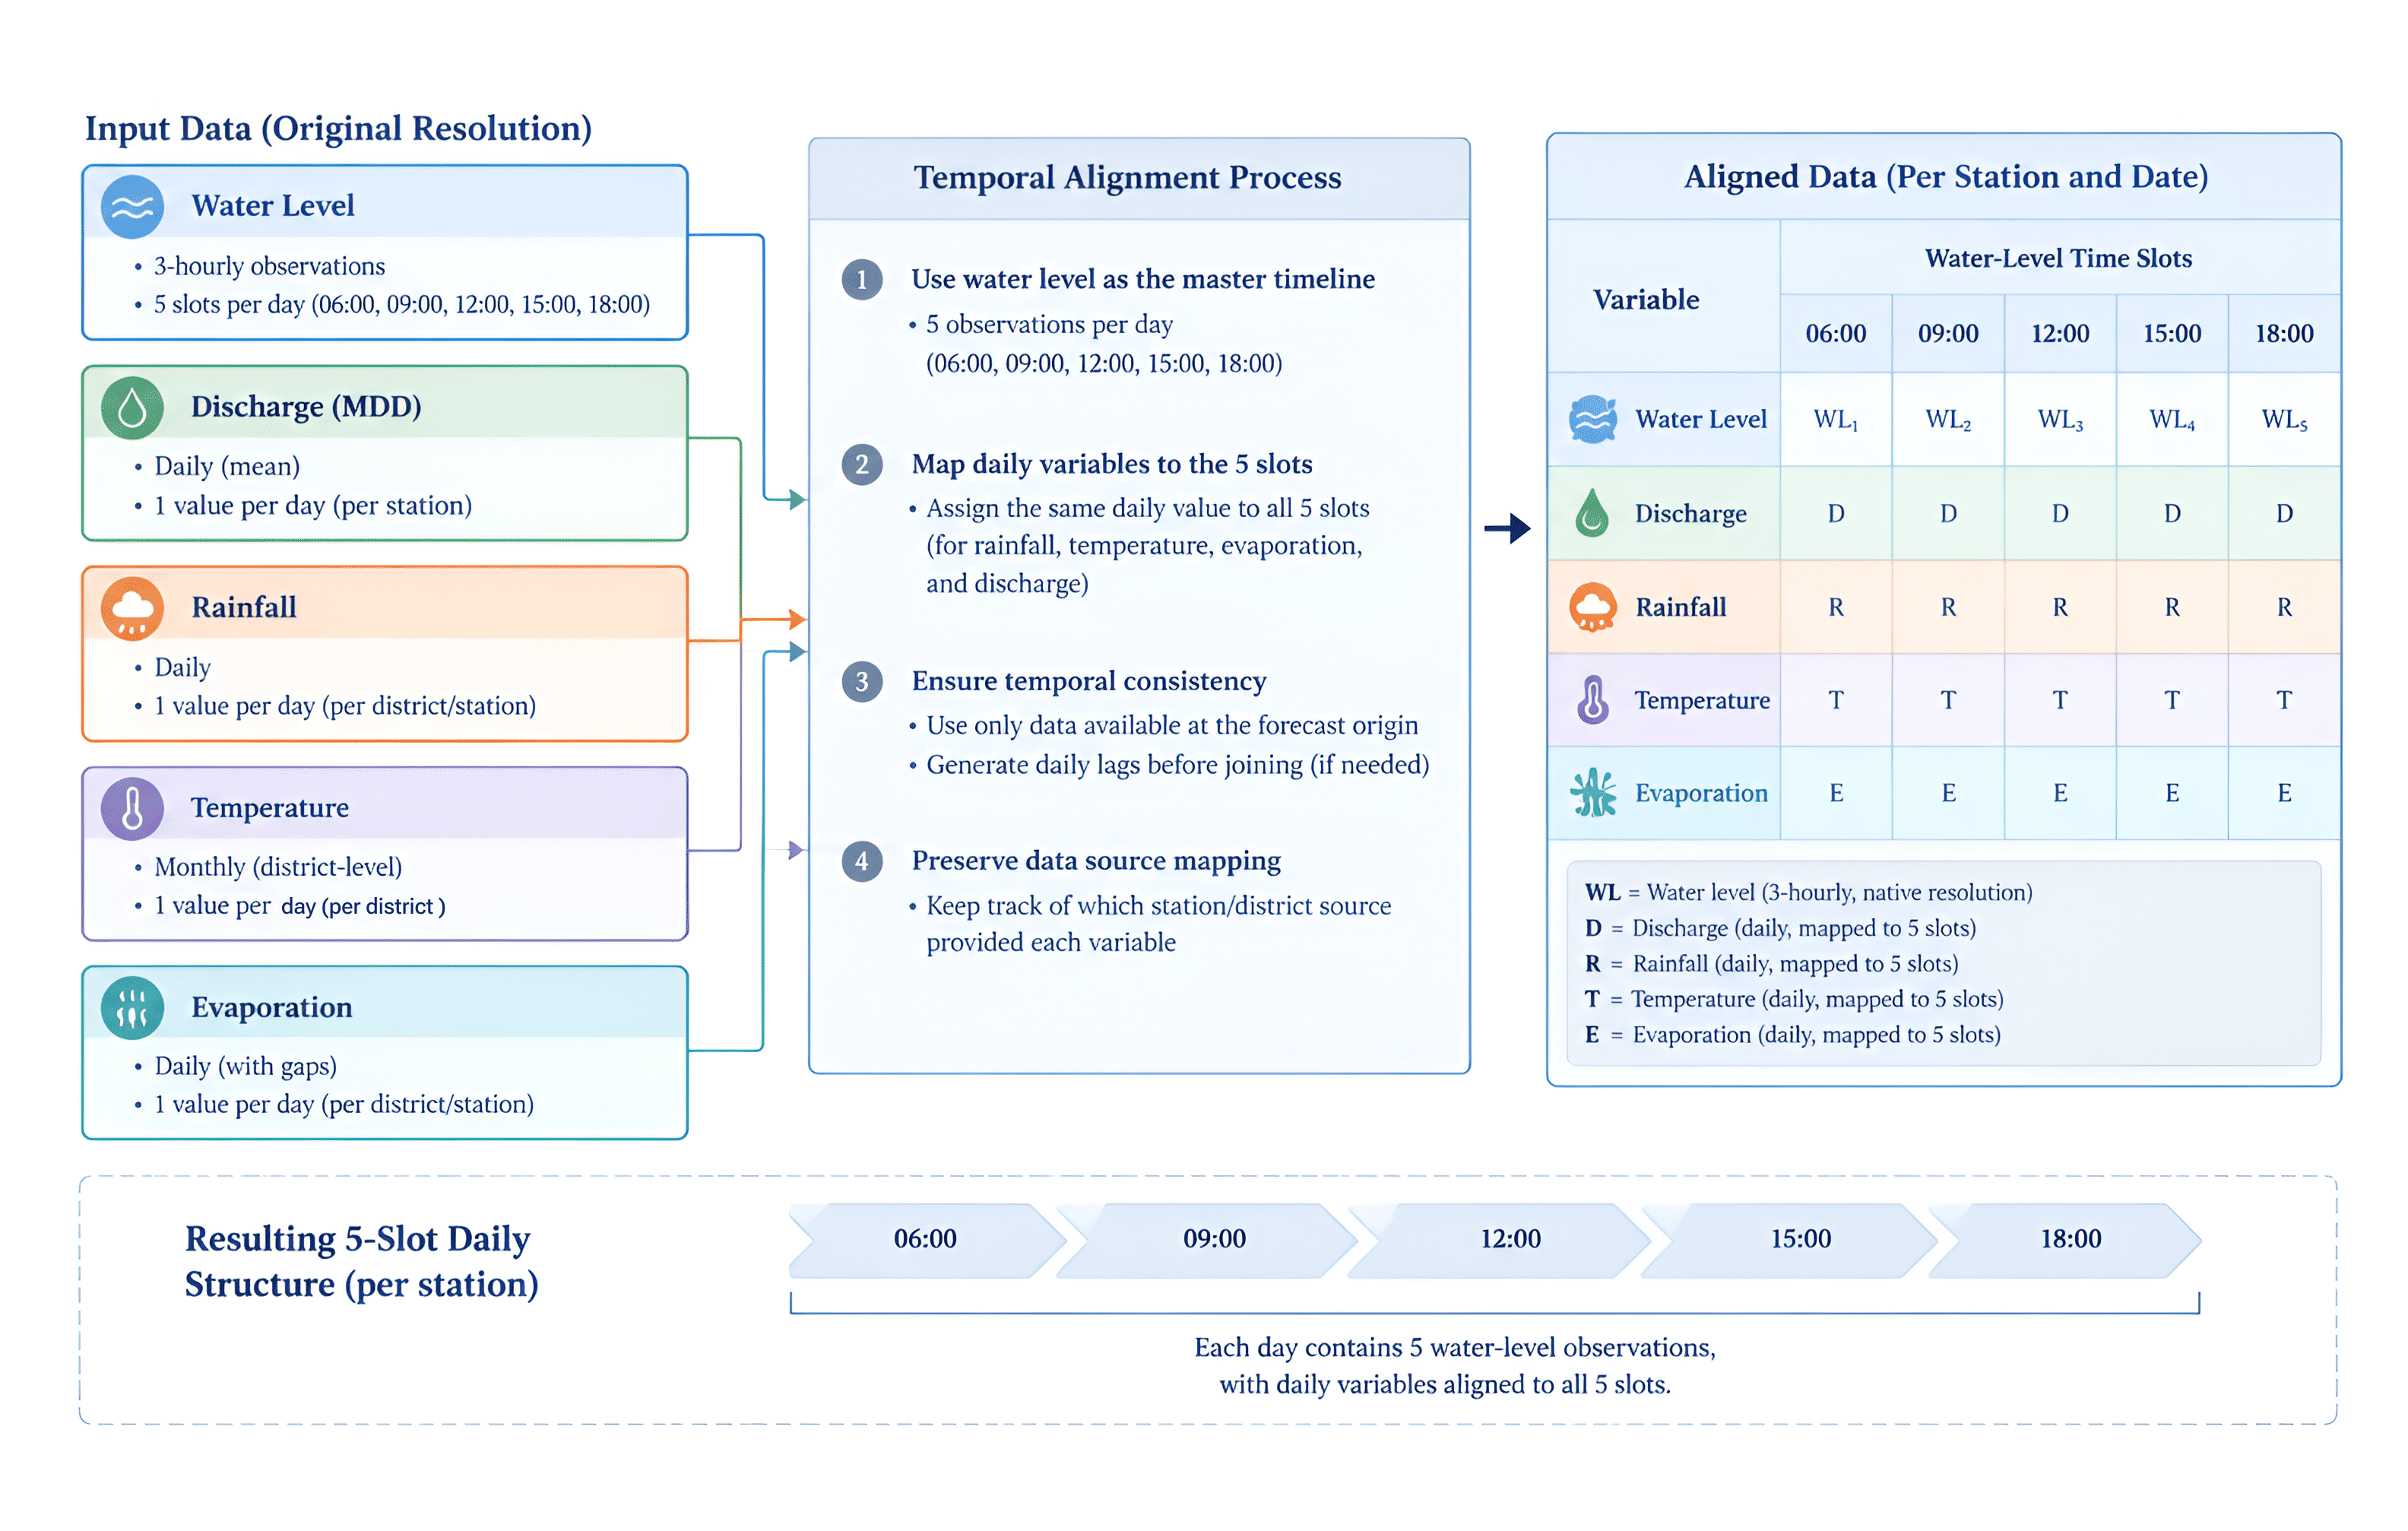
\includegraphics[
        width=0.9\textwidth
    ]{figures2/fig3-5-temporal-alignment.png}

    \caption{Temporal alignment and data-resolution diagram.}
    \label{fig:3.5}
\end{figure}

\begin{table}[htbp]
  \centering
  \caption{Preprocessing Summary}
  \label{tab:3.4}
  \small
  \renewcommand{\arraystretch}{1.2}
  \begin{tabular}{@{}L{2.1cm} L{2.7cm} L{5.1cm} L{3.1cm}@{}}
    \toprule
    \textbf{Variable} & \textbf{Original Resolution} & \textbf{Processing Applied} & \textbf{Final Resolution} \\
    \midrule
    Water Level & 3-hourly, 5 obs/day (06:00--18:00) &
    Retained at native resolution as the master modelling timeline & 5 obs/day (native) \\

    Discharge & Daily (mean) &
    Used directly; trend/rolling features derived; mapped across the 5 WL slots per date &
    Daily value, mapped to 5 WL slots \\

    Rainfall & Daily &
    Used directly; cumulative/lag features derived; mapped across the 5 WL slots per date &
    Daily value, mapped to 5 WL slots \\

    Temperature & Daily, district-level &
    Gaps filled via interpolation; mapped to stations by district; then mapped across the 5 WL slots &
    Daily value, mapped to 5 WL slots \\

    Evaporation & Daily (with gaps) &
    Linearly interpolated to fill gaps; mapped across the 5 WL slots per date &
    Daily value, mapped to 5 WL slots \\
    \bottomrule
  \end{tabular}
\end{table}

\subsection{Normalization}
\label{sec:3.9.4}

Every continuous variable is scaled before it reaches the model, since stable optimization depends on it. Water level, discharge, rainfall, temperature, and evaporation are all scaled separately, since none of them share units or ranges, and the exact method --- standardization or min--max, consistent with the approaches used by \cite{Ruma2023} and \cite{Rakin2023} --- will be chosen once the actual data distributions are in front of us rather than picked in advance. Whether water level needs station-wise scaling is still an open question too; if local baselines differ enough between stations, scaling per station may be worth it, but that decision has to weigh its effect on later cross-station and cross-cluster comparisons, not just on model convergence.

Whatever method is chosen, its parameters are fit on the training data only, then applied unchanged to validation and test. Missingness indicators and station identifiers are left alone rather than scaled as if they were ordinary continuous measurements. Every fitted scaler is saved, predictions are inverse-transformed back into physical units before they're reported, and reconstructed water-level values keep their flag all the way through, so a reconstructed point is never mistaken for a directly observed one downstream.

\subsection{Data Splitting}
\label{sec:3.9.5}

The data is split chronologically, never randomly --- a random split would scatter temporally adjacent, and even future, observations across training and test sets, which defeats the point of a forecasting evaluation. Rather than committing to a single split up front, several chronological configurations are being tried, with the boundary between training, validation, and test moved and re-evaluated to see which split actually yields the most reliable performance, consistent with the chronological (not random) approach used by \cite{Cui2022}. Each candidate boundary is chosen with the same considerations in mind --- what dates are actually available, how station coverage changes across the period, and how flood events are distributed across the timeline --- and whichever configuration is used, it's documented rather than left implicit.

Input and target windows are always built in temporal order, with every target strictly following its input, and the model, scalers, and any imputation parameters are fit using training data alone regardless of which split is being tested. Validation is reserved for model selection, and the test period only ever gets used for a final evaluation. Across all of this, the 15-day horizon (75 water-level observations) is the evaluation point, and errors are reported back in the original water-level units rather than left in scaled form.

\subsection{Feature Engineering}
\label{sec:3.9.6}

Beyond the five raw variables, a set of derived features is built from the cleaned, aligned dataset to make the delayed and cumulative nature of hydrological response more directly visible to the model than the raw series alone would.

\begin{figure}[htbp]
    \centering
    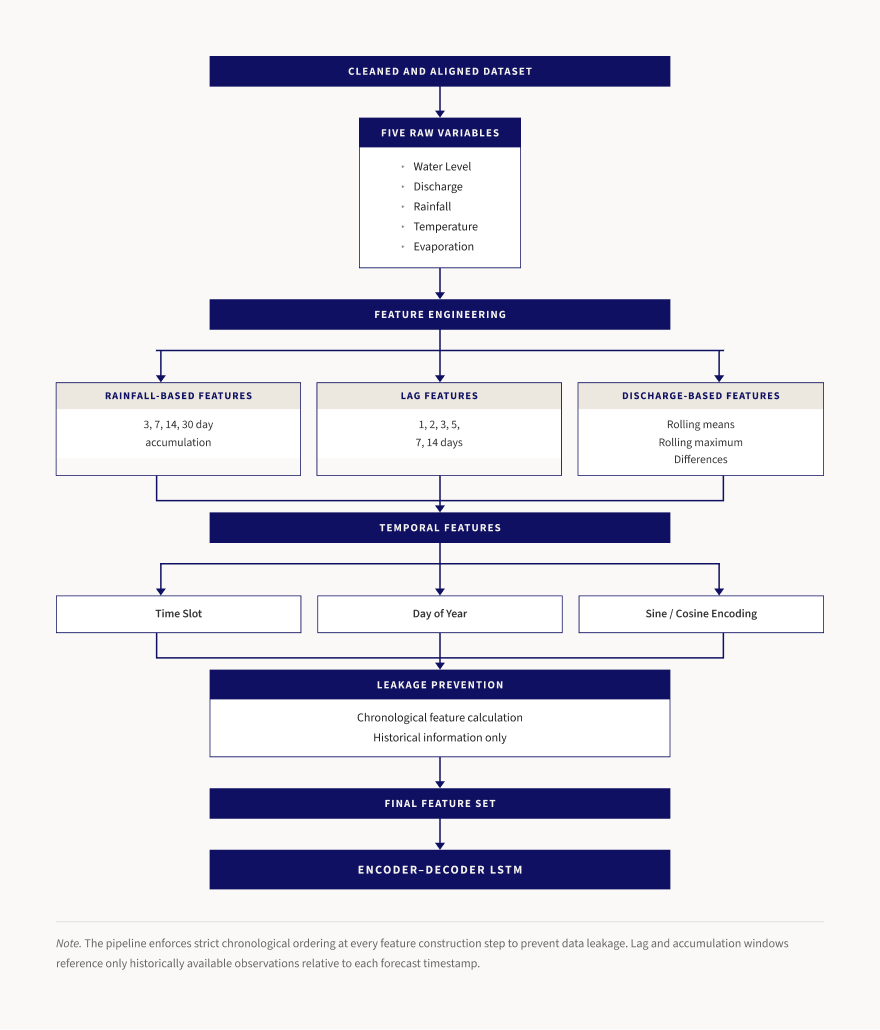
\includegraphics[
        width=0.85\textwidth
    ]{figures2/feature-eng.png}

    \caption{Feature Engineering Workflow}
    \label{fig:3.9.6a}
\end{figure}


\paragraph{Rainfall accumulation.}
To capture how antecedent rainfall builds up before it shows in the river, rainfall is accumulated over look-back windows of 3, 7, 14, and 30 days. For a rainfall series $R$, the accumulated rainfall over the $k$ preceding days is:

\begin{equation}
  R_{\mathrm{acc},k}(t) \;=\; \sum_{i=1}^{k} R(t - i),
  \qquad k \in \{3,\, 7,\, 14,\, 30\}
  \label{eq:3.1}
\end{equation}

which captures both short, sharp rainfall events and longer wet spells, using only rainfall that occurred strictly before the forecast origin.

\paragraph{Lag features.}
Rainfall, discharge, temperature, and evaporation are each given lagged versions at offsets of roughly 1, 2, 3, 5, 7, and 14 days, depending on what the data actually supports, and water-level lags are built from its own preceding observations or matching daily slots. These daily-variable lags are computed on the original daily series first, before that series gets expanded across the five water-level slots --- doing it the other way around would treat five copies of the same value as five independent lags and quietly produce the wrong interval.

\paragraph{Discharge-derived features.}
Recent flow conditions are represented through rolling means of discharge over 3-, 7-, 14-, and, where the data allows, 30-day windows, along with rolling maximum discharge over 7- and 14-day windows to flag recent high-flow periods. One- and three-day discharge differences are also included. None of these are computed where the underlying discharge observations don't meet the completeness rules already set in \S\ref{sec:3.9.2} --- a missing discharge value is never treated as zero for the purpose of building a rolling feature.

\paragraph{Temporal features.}
Calendar and observation-time information is folded in as well --- which of the five daily slots an observation falls in, day of year, and related calendar variables --- with cyclical quantities like time-of-day and day-of-year encoded via sine/cosine transforms. The elapsed time between consecutive observations is also carried through explicitly, given the schedule's own 12-hour overnight gap against the roughly 3-hour daytime gaps established in \S\ref{sec:3.9.3}.

\paragraph{Leakage prevention.}
All of the above is computed strictly chronologically, using only information that would genuinely have been available at each forecast origin. The reporting window of every daily variable is checked specifically for this. The final feature set is decided based on data availability and validation performance, not fixed in advance. The forecasting task itself targets 15 days ahead, or 75 water-level observations under the five-observations-per-day schedule.

% ------------------------------------------------------------
\section{Station Clustering}
\label{sec:3.10}

\subsection{Clustering Criteria}
\label{sec:3.10.1}

Stations were grouped into four clusters using a combination of hydrological/geographic position and a manual cross-check against how stations are actually grouped for operational use on Bangladesh's real-time flood forecasting platform (FFWC). Three factors informed the grouping: position along the river system (upstream tributary, mid-river/mainstem, or downstream distributary reach); proximity to the Dhaka metropolitan area; and, where a station's geographic placement alone was ambiguous, its treatment within FFWC's own operational station groupings, checked and applied manually rather than derived from a statistical clustering algorithm. This domain-knowledge-based approach responds directly to the gap flagged in Chapter~2's review of the general CFL literature \cite{Ghosh2021,Harshvardhan2022,BenAli2026}, none of which were built for a real hydrological network.

\begin{figure}[htbp]
    \centering
    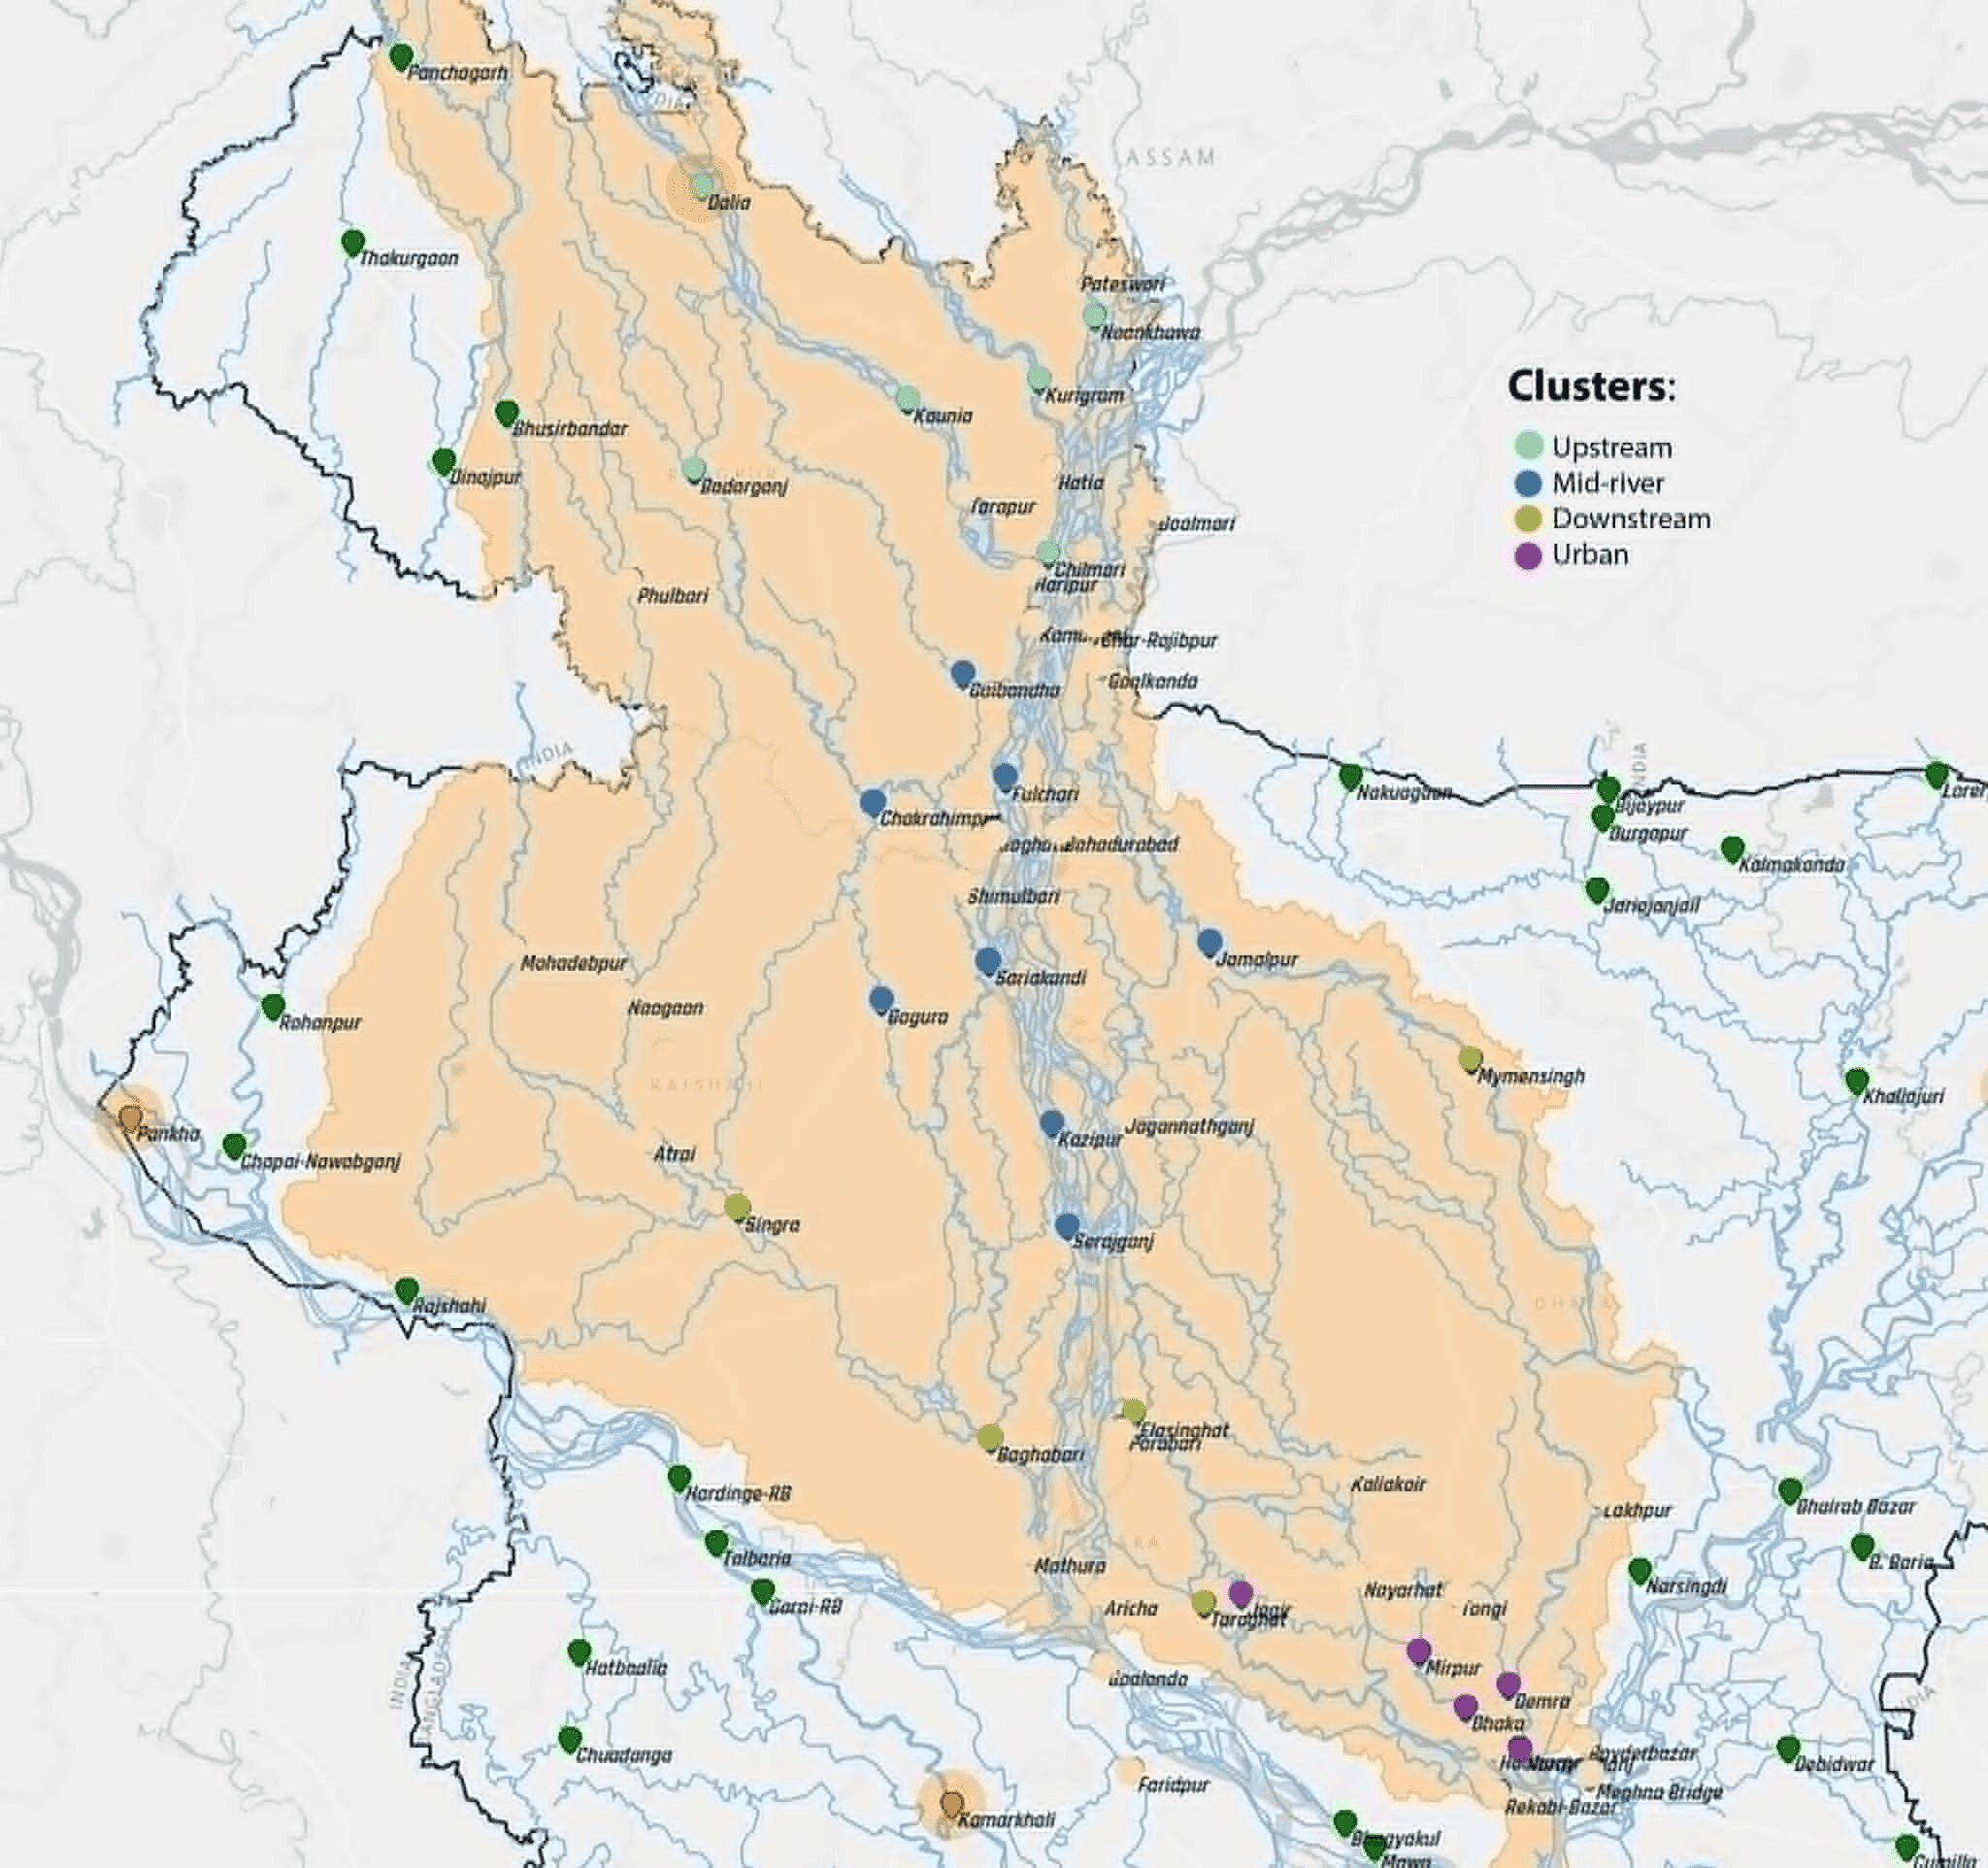
\includegraphics[
        width=0.8\textwidth
    ]{figures2/fig3-6a-cluster-distribution.png}

    \caption{Spatial distribution of the 26 monitoring stations by cluster.}
    \label{fig:3.6}
\end{figure}

\subsection{Cluster Formation and Characteristics}
\label{sec:3.10.2}
The monitoring stations are grouped into four clusters: Upstream, Mid-river, Downstream, and Urban, according to their hydrological and temporal characteristics. This grouping allows the federated learning framework to account for the differences in water-level and flow patterns across stations while learning from stations with similar behavior.

\begin{landscape}
\begin{table}[htbp]
  \centering
  \caption{Cluster Characteristics}
  \label{tab:3.5}
  \footnotesize
  \renewcommand{\arraystretch}{1.25}
  \begin{tabularx}{\linewidth}{@{}L{1.9cm} C{1.4cm} X X L{3.2cm}@{}}
    \toprule
    \textbf{Cluster} & \textbf{Stations} & \textbf{Rivers Represented} &
    \textbf{General Character} & \textbf{Representative Stations} \\
    \midrule
    Upstream & 6 & Teesta, Dharla, Deonai-Charalkata-Jamuneswari-Karatoa, Brahmaputra-Jamuna &
    Northernmost stations; non-tidal; closest to the point where flow enters Bangladesh from upstream catchments &
    Dalia, Kaunia, Kurigram \\

    Middle & 8 & Deonai-Charalkata-Jamuneswari-Karatoa, Ghagot, Brahmaputra-Jamuna, Old Brahmaputra &
    Central mainstem stations, largest cluster by station count; non-tidal &
    Bogra, Sirajganj, Jamalpur \\

    Downstream & 5 & Karatoa-Atrai-Gur-Gumani-Hurasagar, Old Brahmaputra, Dhaleswari, Kaliganga-Bethua &
    Distributary and secondary-channel reaches south of the main confluence zone; non-tidal &
    Baghabari, Mymensingh, Elashin \\

    Urban & 6 & Dhaleswari, Buriganga, Turag, Lakhya, Balu &
    Mostly Dhaka-metropolitan and tidally influenced (5 of 6 stations are Tidal-type --- the only Tidal stations in the dataset) &
    Dhaka (Mill Barrack), Mirpur, Narayanganj \\
    \bottomrule
  \end{tabularx}
\end{table}
\end{landscape}


% ------------------------------------------------------------
\section{Time-Series Input \& Forecasting Setup}
\label{sec:3.11}

Each model is trained on a sliding window of the past 30 days of daily observations across all five variables --- under the five-observations-per-day water-level schedule established in \S\ref{sec:3.9.3}, a 30-day input window corresponds to 150 water-level observations --- and asked to forecast water level at seven horizons: 3 hours, 6 hours, 12 hours, 1 day, 3 days, 7 days, and 15 days ahead, with the 15-day horizon corresponding to 75 water-level observations. Evaluating this wide a horizon range from a single 30-day input window is, as established in Chapter~2, wider than anything in the reviewed literature --- the closest precedents \cite{Kao2020,Cui2022} stop at 12 hours, and \cite{Islam2026a} reaches 30 days but only for discharge, at two stations, without any federated or clustered component.

\begin{figure}[htbp]
    \centering

    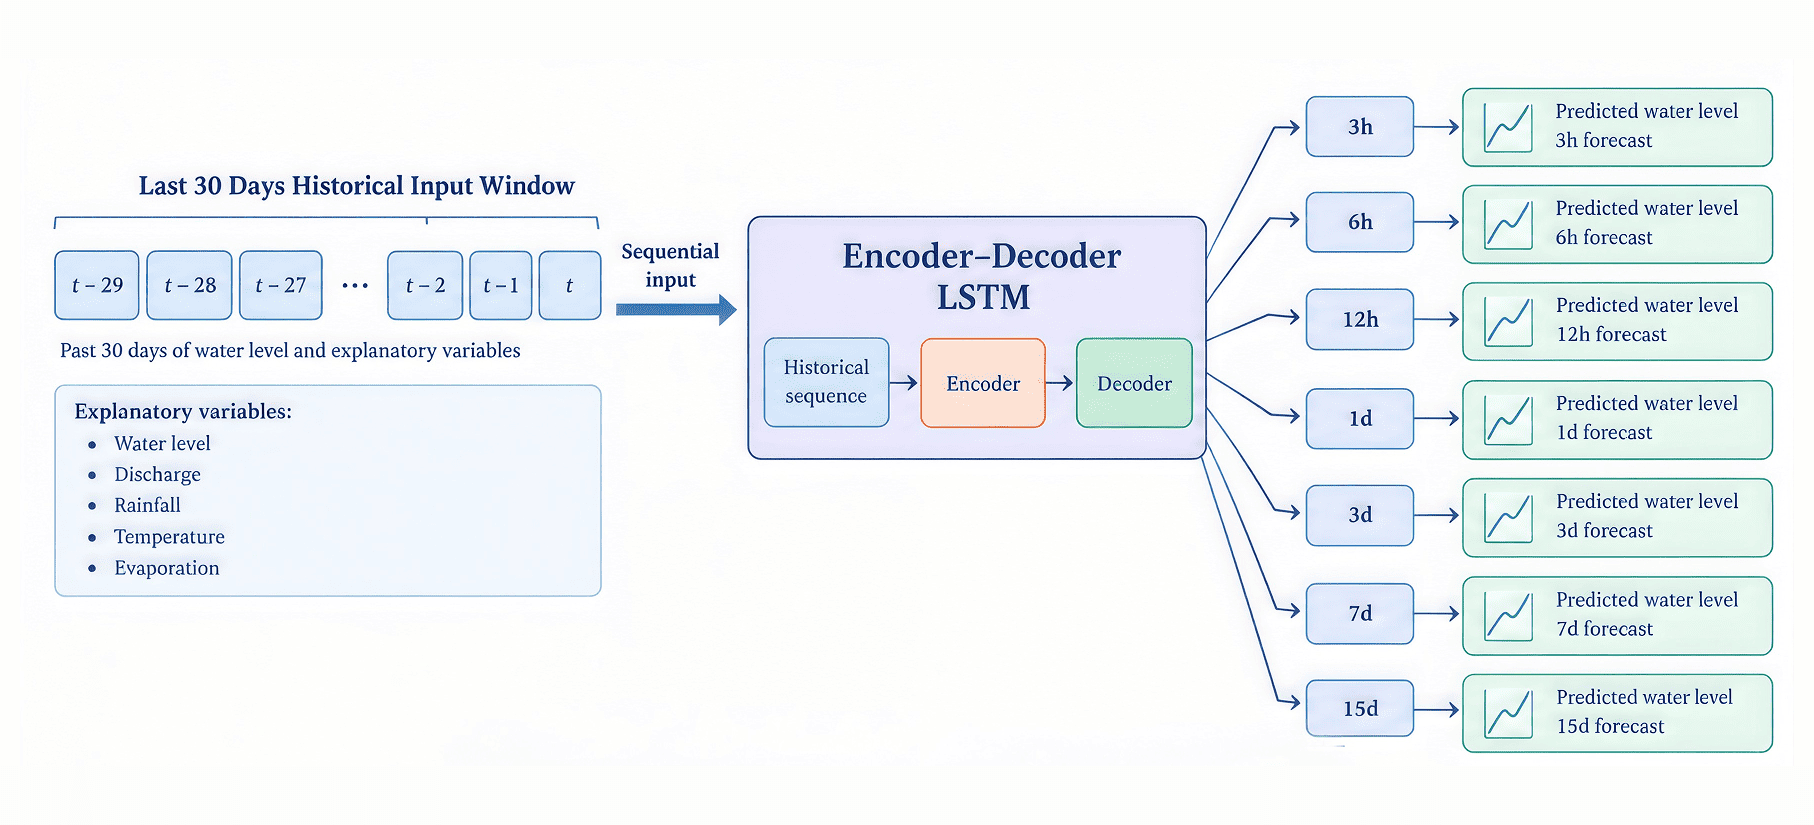
\includegraphics[
        width=0.9\textwidth
    ]{figures2/fig3-7-window-diagram.png}

    \caption{Time-series input/output window diagram.}
    \label{fig:3.7}
\end{figure}